\section{Timing Diagrams}
The timing diagram for the testbench is shown in Figure$^{\ref{simulation_image}}$

% \lipsum[1-5]
\begin{figure}[H]
  \centering
  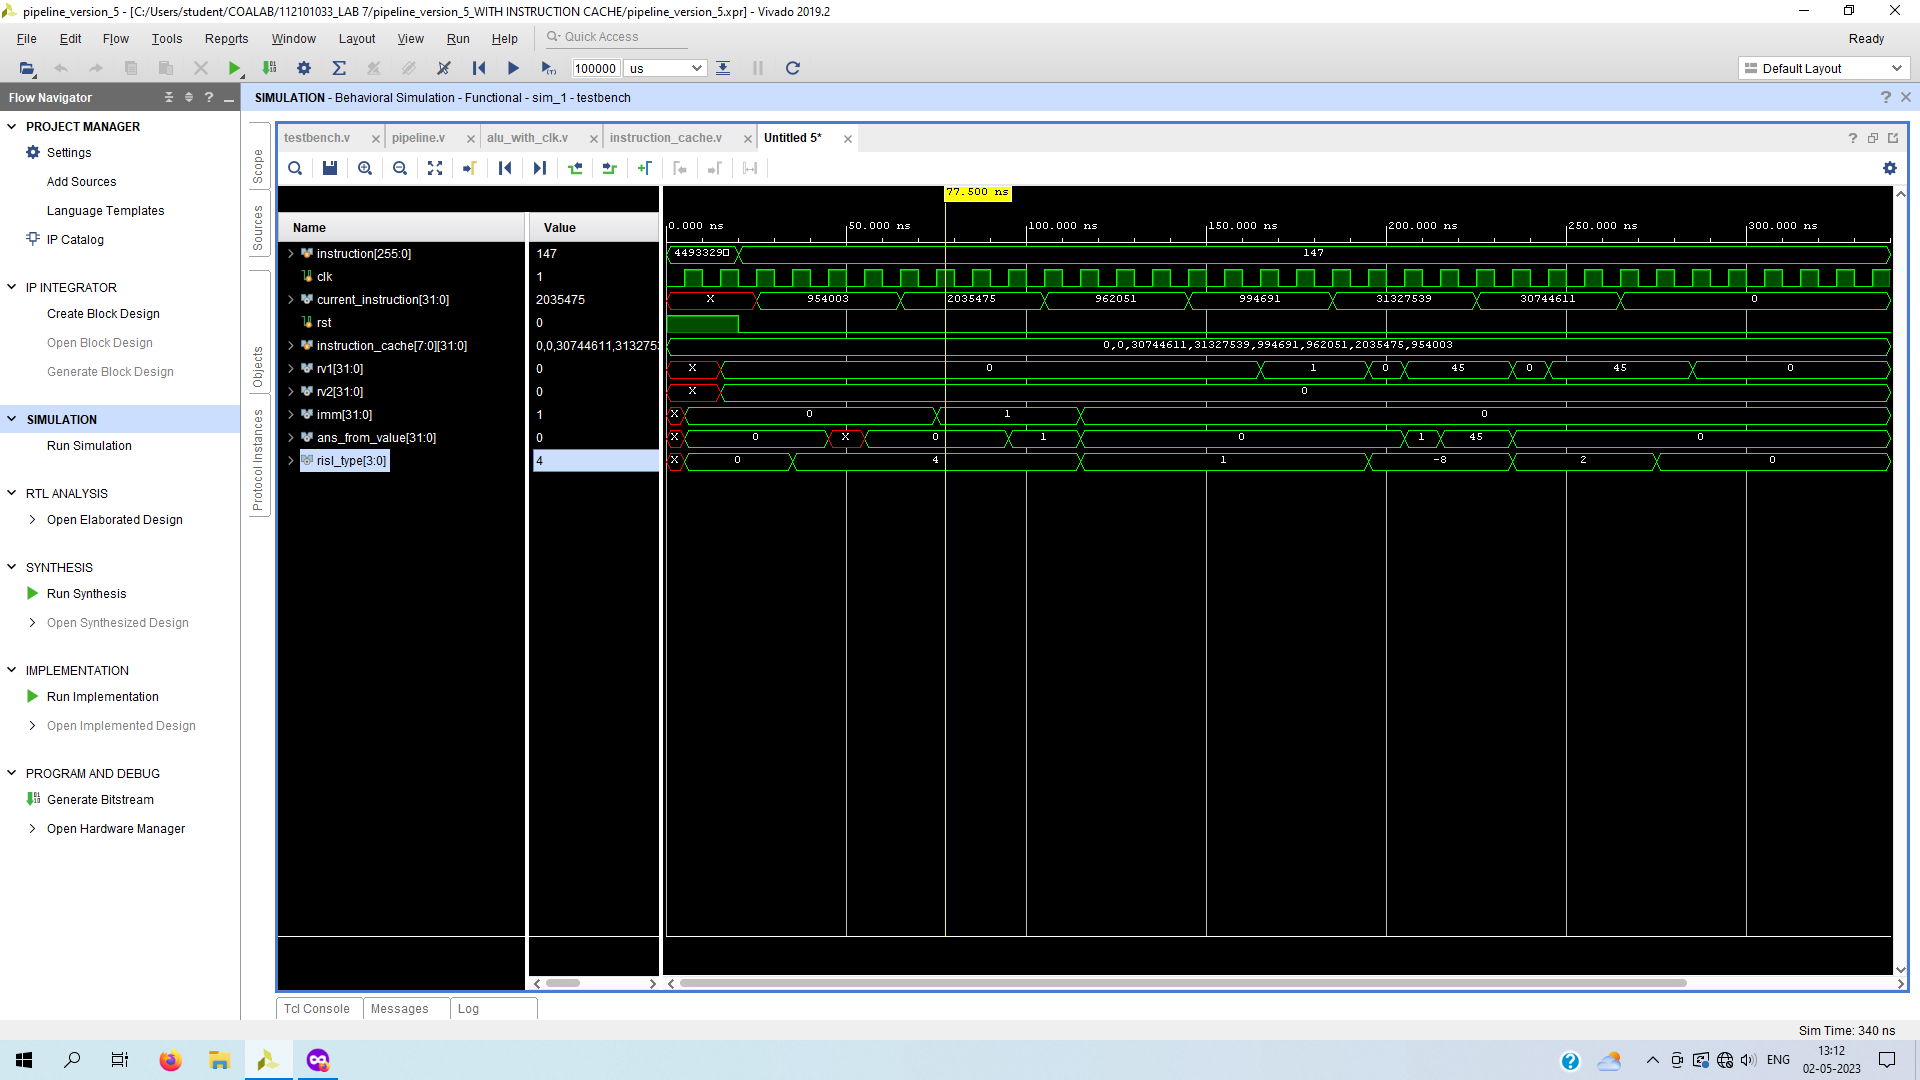
\includegraphics[width=\textwidth]{./images/simulation_lab_7.png}
  \caption{Simulation of Testbench}
  \label{simulation_image}
\end{figure}
% \lipsum[1-3]
In the timing diagram, at the first posedge clk after \textbf{rst becomes zero}, the first instruction is fetched as shown by the \textbf{current\textunderscore instruction} in the simulation image$^{\ref{simulation_image}}$ and it completes it in 4 clock cycles, and the subsequent instruction is fetched and this goes on till the program counter reaches the end of the instruction.
\begin{itemize}
  \item The read value 1 is shown as rv1.
  \item The read value 2 is shown as rv2.
  \item The immediate value is shown as imm.
\end{itemize}